\scanpage{26}

\figure{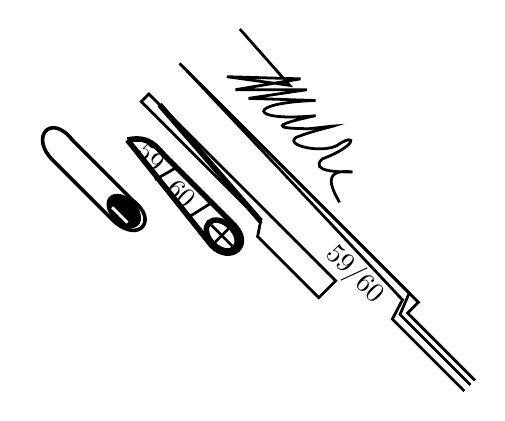
\begin{tikzpicture}[x=.55cm,y=.55cm,line width=1pt]
\begin{scope}[rotate=-45]
\draw (0,1)--(7.5,1)--(7.7,.5)--(10,.5);\draw (.25,1)--(7.5,.78)--(7.65,.3)--(10,.3);\draw (.65,1)--(7.8,1)--(7.8,.65)--(10,.65);
\draw (0,0)--(6.1,0)--(6.1,-.55)--(4.1,-.55)--(3.9,-.25)--(0,-.25)--cycle;
\draw[line width=2pt] (.35,0)--(3.9,-.25);\node[rotate=-45] at (6.3,.4) {$59/60$};
\draw[line width=2pt] (.4,-1.1) .. controls (.7,-.65) and (1,-.75) .. (1.3,-.75)--(3.5,-.75) .. controls (4.2,-.75) and (4.1,-1.45) .. (3.5,-1.45)--(.4,-1.1);
\draw (1.65,-.75)--(1.5,-1.3);\draw (2.8,-.75)--(2.65,-1.4);
\node[rotate=-45] at (1.05,-1) {$\unsure{59}$};\node[rotate=-45] at (2.15,-1.1) {$60$};
\draw[line width=2pt] (3.5,-1.12) ellipse (.42 and .28);\draw (3.15,-1.12)--(3.85,-1.12);\draw (3.5,-.86)--(3.5,-1.38);
\draw[line width=1.3pt] (-.5,-2) .. controls (-1.3,-1.9) and (-1.25,-2.65) .. (-.5,-2.65)--(1.5,-2.65) .. controls (2.3,-2.6) and (2.2,-1.9) .. (1.5,-2)--cycle;
\fill (1.5,-2.32) ellipse (.47 and .31);\draw[white] (1.25,-2.45)--(1.75,-2.45);
\end{scope}
\draw (2.1,1.5)--(3.25,.2)--(1.8,.4)--(3.5,.35)--(2,.1)--(3.65,.1)--(2.3,-.1)--(3.85,-.15) .. controls (2.2,-.2) and (2.3,-.65) .. (3.85,-.5) .. controls (2.9,-.7) and (2.8,-.8) .. (3.7,-.8) .. controls (4.7,-.7) and (4.2,-.7) .. (3.4,-1) .. controls (3.1,-1.2) and (4.1,-1.4) .. (4.4,-1.15) .. controls (4.8,-.9) and (4.8,-1.2) .. (4,-1.5) .. controls (3.7,-1.8) and (4.4,-1.8) .. (4.7,-1.8) .. controls (3.9,-1.7) and (4.3,-2.3) .. (4.4,-2.5);
\end{tikzpicture}}

\begin{center}$-\ 11\ -$\end{center}\hfill n\textsuperscript{o} 276

et par conséquent :
\[
a_n-\sum_{i=0}^{i=i_p}a_{in}\in\mathrm m^{p-n}.
\]
Considérant alors la série formelle $y=\sum a_nX^n$, la relation précédente montre que l'on a
\[
y-\sum_{i=0}^{i=i_p}y_i\in\mathrm n^p
\]
ce qui prouve que la série $\sum y_i$ converge vers $y$, d'où la proposition.

\uline{Corollaire} -- \uline{Soit} $A$ \uline{un anneau commutatif}. \uline{L'anneau de séries formelles} $A[[X_1,\ldots,X_r]]$ \uline{filtré par les puissances de l'idéal} $(X_1,\ldots X_r)$, \uline{est séparé et complet}.

5. -- \uline{Modules de type fini sur un anneau filtré complet}.

Soient $(E,E_n)$ et $(F,F_n)$ deux modules filtrés sur un anneau filtré $(A,A_n)$ par un \uline{homomorphisme} $u:(E,E_n)\longrightarrow(F,F_n)$ on entendra tout homomorphisme $u:E\longrightarrow F$ de $A$-modules, tel que l'on ait
\[
u(E_n)\subset F_n
\]
pour tout $n$. Si les filtrations de $E$ et $F$ sont associées à la filtration donnée de $A$, tout homomorphisme de $A$-modules est un homomorphisme de modules filtrés.

Il est clair que tout homomorphisme $u:(E,E_n)\longrightarrow(F,F_n)$ définit canoniquement un homomorphisme $G(u):G(E)\longrightarrow G(F)$ des $G(A)$-modules gradués associés, obtenu par passage au quotient.

PROPOSITION 6 -- \uline{Soient} $(E,E_n)$ \uline{et} $(F,F_n)$ \uline{deux modules filtrés sur un anneau filtré}, \uline{et} $u:(E,E_n)\longrightarrow(F,F_n)$ \uline{un homomorphisme de modules filtrés}. \uline{Supposons remplies les conditions suivantes} :

a) : $(E,E_n)$ \uline{est complet}.

b) : $(F,F_n)$ \uline{est séparé}.

c) : \uline{l'homomorphisme associé} $G(u)$ \uline{est surjectif}.
\mspage{25}
